\documentclass{beamer}
\usepackage{lmodern}
\usepackage{hyperref}
\beamertemplatenavigationsymbolsempty

\title{SIAM-IMA Etymo workshop - text extraction}
\author{Steven Elsworth}
\date{June 13, 2018}

\begin{document}
\maketitle

\begin{frame}
 \frametitle{\centerline{Text extraction}}
 \begin{figure}[h]
\centering
\begin{minipage}{0.45\textwidth}
\centering
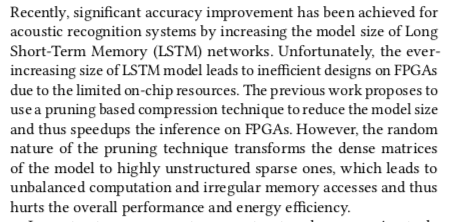
\includegraphics[scale=0.3]{img/pdf_paragraph}
\end{minipage}
\begin{minipage}{0.45\textwidth}
\centering
\tiny
Recently, significant accuracy improvement has been achieved for acoustic recognition systems by increasing the model size of Long Short-Term Memory (LSTM) networks. Unfortunately, the ever- increasing size of LSTM model leads to inefficient designs on FPGAs due to the limited on-chip resources. The previous work proposes to use a pruning based compression technique to reduce the model size and thus speedups the inference on FPGAs. However, the random nature of the pruning technique transforms the dense matrices of the model to highly unstructured sparse ones, which leads to unbalanced computation and irregular memory accesses and thus hurts the overall performance and energy efficiency.
\end{minipage}
\end{figure}
\end{frame}

\begin{frame}
\frametitle{Methods}
\begin{itemize}
\item pdftotxt
\vspace{0.2cm}
\item Textract (Backend pdftotxt)
\vspace{0.2cm}
\item PyPDF2
\vspace{0.2cm}
\item pdfminer
\vspace{0.2cm}
\item pyocr (backend tesseract)
\end{itemize}

\vspace{1cm}
See Jupyter Notebook.
\end{frame}

\begin{frame}
\frametitle{Problems faced}

Give examples of :
\begin{itemize}
\item Equation conversion
\item Figure conversion
\item White space
\item Merged words
\item Page Columns
\item Time
\end{itemize}
\end{frame}
\end{document}
